%! TeX program = lualatex
\documentclass[a4paper,11pt]{article} 
% packages
\usepackage{censor}
\StopCensoring
\usepackage{fontspec}
\setmainfont{EB Garamond}
% for tironian et fallback
% % \directlua{luaotfload.add_fallback
% % ("emojifallback",
% %      {"Noto Serif:mode=harf"}
% % )}
% % \setmainfont{EB Garamond}[RawFeature={fallback=emojifallback}]

\setmonofont[Scale=MatchLowercase]{Deja Vu Sans Mono}
\usepackage[a4paper,left=2cm,right=2cm,top=\dimexpr15mm+1.5\baselineskip,bottom=2cm]{geometry}
\setlength{\parindent}{0pt}

\usepackage{fancyhdr}       % Headers and footers 
\fancyhead[R]{\normalfont \leftmark}
\fancyhead[L]{}
\pagestyle{fancy}

\usepackage{microtype}      % Slightly tweak font spacing for aesthetics
\usepackage[english]{babel} % Language hyphenation and typographical rules
\usepackage{xcolor}
\definecolor{linkblue}{RGB}{0, 64, 128}
\usepackage[final, colorlinks = false, urlcolor = linkblue]{hyperref} 
% \newcommand{\secref}[1]{\textbf{§~\nameref{#1}}}
\newcommand{\secref}[1]{\textbf{§\ref{#1}~\nameref{#1}}}
\usepackage{array}
\usepackage{amsmath}

\usepackage{changepage}     % adjust margins on the fly


\usepackage{minted}
\usemintedstyle{algol_nu}

\usepackage{pgfplots}
\pgfplotsset{width=\textwidth,compat=1.9}

\usepackage{caption}
\newenvironment{code}{\captionsetup{type=listing}}{}
\captionsetup[listing]{skip=0pt}
\setlength{\abovecaptionskip}{5pt}
\setlength{\belowcaptionskip}{5pt}

\usepackage[yyyymmdd]{datetime}
\renewcommand{\dateseparator}{--}

\usepackage{enumitem}

\usepackage{titlesec}

\author{Andrew Hayes}

\begin{document}
\begin{titlepage}
    \begin{center}
        \hrule
        \vspace*{0.6cm}
        \huge \textbf{CT417}
        \vspace*{0.6cm}
        \hrule
        \LARGE
        \vspace{0.5cm}
            Software Engineering III
        \vspace{0.5cm}
        \hrule

        \vfill
        \vfill

        \hrule
        \begin{minipage}{0.495\textwidth} 
            \vspace{0.4em}
            \raggedright
            \normalsize 
            Name: Andrew Hayes \\
            E-mail: \href{mailto://a.hayes18@universityofgalway.ie}{\texttt{a.hayes18@universityofgalway.ie}}  \hfill\\
            Student ID: 21321503 \hfill
        \end{minipage}
        \begin{minipage}{0.495\textwidth} 
            \raggedleft
            \vspace*{0.8cm}
            \Large
            \today
            \vspace*{0.6cm}
        \end{minipage}
        \medskip\hrule 
    \end{center}
\end{titlepage}

\pagenumbering{roman}
\newpage
\tableofcontents
\newpage
\setcounter{page}{1}
\pagenumbering{arabic}

\section{Introduction}
\subsection{Lecturer Contact Details}
\begin{itemize}
    \item   Dr. Effirul Ramlan.
    \item   Email: \href{mailto://effirul.ramlan@universityofgalway.ie}{\texttt{effirul.ramlan@universityofgalway.ie}}.
    \item   Will attempt to reply to emails immediately between the hours of 09:00 \& 20:00 from Week 01 to
            Week 12.
    \item   Discord server: \url{https://discord.gg/CRAtHv9uNg}.
\end{itemize}

\subsection{Grading}
\begin{itemize}
    \item   Continuous Assessment: 40\%.
            \begin{itemize}
                \item   You will work in pairs on a software project with three key submissions across the 12 weeks.
                        Each deliverable will align with the topics covered in the course up to that point, allowing 
                        for continuous progress assessment.
                \item   AS-01: Set up musicFinder and configure the CI/CD pipeline (Week 4).
                \item   AS-02: Testing, Security, \& Expanded Application (Week 8).
                \item   AS-03: Refactoring \& Application Deployment.
            \end{itemize}

    \item   Final Exam: 60\%.
            \begin{itemize}
                \item   Typical 2-hour exam paper covering materials from Week 1 to Week 12, with nothing out of the ordinary --
                        ``You can be sure of that''.
                    \item   ``There is a question on Agile on your final'' -- key differences between agile \& DevOps table.
            \end{itemize}
\end{itemize}

\section{Revision}
\subsection{What is Software?}
\textbf{Software} consists of:
\begin{enumerate}[label=\roman*.]
    \item   Instruction (computer programs) that when executed provide desired features, function, \& performance.
    \item   Data structures (Arrays, Objects, Lists, Dictionaries, Maps, etc.) that enable programs to manipulate information.
    \item   Descriptive information in both hard copy \& virtual format describing the operation \& use.
\end{enumerate}

\subsection{Functional vs Non-Functional Requirements}
\begin{table}[h!]
    \centering

    \begin{tabular}{|>{\arraybackslash}p{0.5\textwidth}|>{\arraybackslash}p{0.5\textwidth}|}
        \hline
        \textbf{Functional Requirement}                                             & \textbf{Non-Functional Requirement} \\
        \hline
        Describes the actions with which the user's work is concerned               & Describes the experience of the user while doing the work \\
        \hline
        A feature or function that can be captured in use-cases                     & A global constraint (and therefore difficult to capture in use-cases) \\
        \hline
        A behaviour that can be analysed via sequence diagrams or state machines    & A software quality \\
        \hline
        can be usually traced back to a single module / class / function            & Usually cannot be implemented in a single module or even program \\
        \hline
    \end{tabular}
    \caption{Functional vs Non-Functional Requirements}
\end{table}

Typical non-functional requirements include: availability, maintainability, performance, privacy, reliablility, scalability, \& security.

\subsection{What is Software Engineering?}
\textbf{Software Engineering} is the field of computer science that deals with the building of software systems that are so large or so complex
that they are built by a team or teams of engineers.
Software Engineering encompasses a process, a collection of methods, \& an array of tools that allow professionals to build high-quality software.
\\\\
\textbf{DevOps} outlines a software development process that increases the delivery of higher quality software by integrating the efforts of the development 
\& IT operation teams.
$$
    \text{DevOps} = \text{Software Engineering} + \text{IT Operations}
$$

\subsection{What are Software Development Life Cycles?}
\textbf{Software Development Life Cycles (SDLC)} refers to a process used by software engineers to design, develop, \& test software.
Each approach focuses on a different aspect of development, from planning to continuous improvement.

\subsection{What is a Framework?}
A \textbf{software framework} is an abstraction in which common code providing generic functionality can be selectively 
overridden or specialised by user providing specific functionality.
\\\\
\textbf{Low-code} is a method of designing \& developing applications using an intuitive GUI \& embedded functionality that reduce 
traditional professional code writing requirements.
\textbf{No-code} is similar to low-code, but for non-technical business users as it allows them to develop software / applications without
having to write a single line of code.

\subsection{Agile \& DevOps}
\subsubsection{What is Agile?}
\textbf{Agile} is a method of software development consisting of:
\begin{itemize}
    \item   \textbf{Iterative \& Incremental Development:} Software is developed in small, workable increments.
    \item   \textbf{Customer-Centric:} Constant feedback from customers to refine requirements.
    \item   \textbf{Frequent Delivery:} Rapid releases of smaller, functional product versions.
    \item   \textbf{Adaptability:} Agile responds to change quickly
\end{itemize}

\subsubsection{Agile Principles}
\begin{itemize}
    \item   \textbf{Individuals \& Interactions:} over processes \& tools.
    \item   \textbf{Working Software:} over comprehensive documentation.
    \item   \textbf{Customer Collaboration:} over contract negotiation.
    \item   \textbf{Responding to Change:} over following a plan.
    \item   \textbf{Quote:} ``The highest priority is to satisfy the customer through early \& continuous delivery of valuable software.''
\end{itemize}

\subsubsection{Agile Frameworks}
Agile methodologies \& frameworks include:
\begin{itemize}
    \item   \textbf{Scrum:} Divides work into sprints (2-4 weeks) with regular stand-ups \& reviews.
    \item   \textbf{Kanban:} Focuses on visualising workflow \& limiting Work-In-Progress (WIP).
    \item   \textbf{XP (eXtreme Programming):} Emphasises technical excellence \& frequent releases.
    \item   \textbf{Lean Development:} Focuses on minimising waste \& maximising value.
\end{itemize}

\subsubsection{What is DevOps?}
\textbf{DevOps} is a culture \& set of practices that integrated development (Dev) \& operations (Ops).
It involves collaboration \& automation between developers \& IT operations for faster delivery of high-quality software.
It also involves continuous integration/continuous delivery (CI/CD) to automate code testing \& deployment.

$$
    \text{DevOps} = \text{Development} + \text{Operations}
$$

\subsubsection{DevOps Core Practices}
DevOps core practices include:
\begin{itemize}
    \item   \textbf{CI/CD Pipelines:} Automating the building, testing, \& deployment of code.
    \item   \textbf{Infrastructure as Code (IaC):} Managing infrastructure through code (e.g., Terraform, Ansible).
    \item   \textbf{Monitoring \& Logging:} Ensures system reliability through real-time tracking \& analysis.
    \item   \textbf{Collaboration \& Communication:} Cross-functional teams sharing ownership of development \& operations tasks.
\end{itemize}

\subsubsection{Key Differences between Agile \& DevOps}
\begin{table}[h!]
    \centering

    \begin{tabular}{|>{\arraybackslash}p{0.5\textwidth}|>{\arraybackslash}p{0.5\textwidth}|}
        \hline
        \textbf{Agile}                                                              & \textbf{DevOps} \\
        \hline
        Focus on frequent customer feedback                                         & Focus on collaboration between Dev \& Ops teams \\
        \hline
        Iteration done through iterative cycles                                     & Iteration done through rapid feedback loops \\
        \hline
        Scope of smaller, incremental changes                                       & Scope of large-scale projects \\
        \hline
        Uses task management software (e.g. Jira)                                   & Uses automation tools (e.g. Jenkins) \\
        \hline
        Scrum, XP frameworks                                                        & Kanban, DevOps lifecycle frameworks \\
        \hline
    \end{tabular}
    \caption{Key Differences between Agile \& DevOps}
\end{table}

\textbf{Agile} focuses on iterative development \& customer feedback, with a short feedback loop.
\textbf{DevOps} focuses on automating delivery, collaboration, \& integration between Dev \& Ops teams, integrating the entire process for faster releases.

\subsubsection{Why DevOps Complements Agile}
Agile improvements development velocity, but DevOps extends the concept to deployment \& maintenance.
Both are customer-focused, but DevOps ensures rapid \& reliable deployment in addition to development.
DevOps fills gaps Agile doesn't cover, like operations, infrastructure, \& automation.
Agile helps development teams iterate \& adapt to changing requirements, while DevOps bridges the gap between developers \& IT operations.

\subsubsection{Benefits of Agile \& DevOps}
\begin{itemize}
    \item   Faster, more frequent delivery of features.
    \item   Improved communication \& collaboration between teams. 
    \item   Reduced risk of deployment errors.
    \item   Ability to adapt to customer feedback \& market changes rapidly.
    \item   Higher-quality software \& reduced time-to-market.
\end{itemize}
 
\section{Version Control}
\subsection{What is Version Control?}
\textbf{Version Control} is a system that records changes to a file or set of files over time, allowing you to recall or access specific versions
at a later date.
It is also known as \textit{revision control} or \textit{source control}.
It allows you to keep track of changes, by whom, \& when they occurred.
Some of the popular version control programs include Git, CVS, Subversion, Team Foundation Server, \& Mercurial.
\\\\
It allows us to:
\begin{itemize}
    \item   Backup the source code and be able to rollback to a previous version.
    \item   Keep a record of who did what and when (know who to praise \& who to fire).
    \item   Collaborate with the team (know who to praise \& who to fire).
    \item   Troubleshoot issues by analysing the change history to figure out what caused the problem.
    \item   Analyse statistics such as who is being the most productive etc.
\end{itemize}

\subsection{What files should be checked in to Version Control?}
Any file that influences the software build should be checked into version control.
This includes configuration files, file encodings, binary settings, etc.
Furthermore, anything that is needed to setup the project from a clean checkout / fork should also be included in the version 
control, such as source code, documentation, manuals, image files, datasets, etc.
\\\\
You should not check in any binary files such as JAR files or any other ``build'' files, any intermediate files from build / 
compilation such as \verb|.pyc| or \verb|.o| files, any files which contain an absolute path, or personal preference /
personal settings files.

\subsection{Centralised Version Control -- Subversion}
\begin{figure}[H]
    \centering
    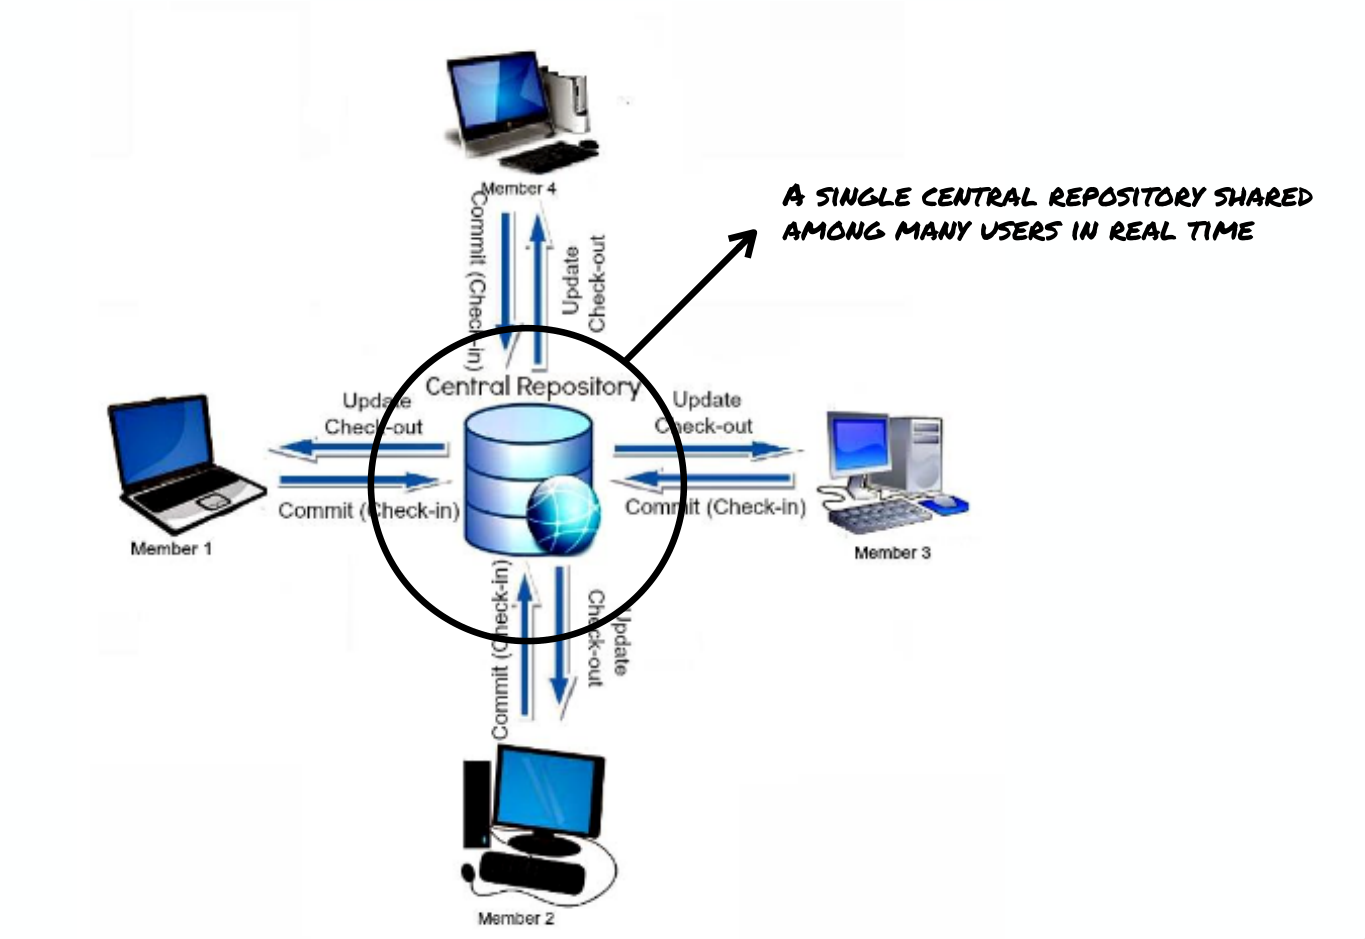
\includegraphics[width=0.8\textwidth]{images/centralised_vcs.png}
    \caption{Centralised Version Control System Diagram}
\end{figure}

\textbf{Subversion} is a centralised version control system in which code is centralised in a repository which can be checked out 
to get a working copy on your local machine.
In general, you don't have the entire repository checked out in Subversion, just a specific branch.
Changes are committed back to the central repository, ``normally'' with useful comments, and a change log is maintained 
of who did what \& when.

\begin{figure}[H]
    \centering
    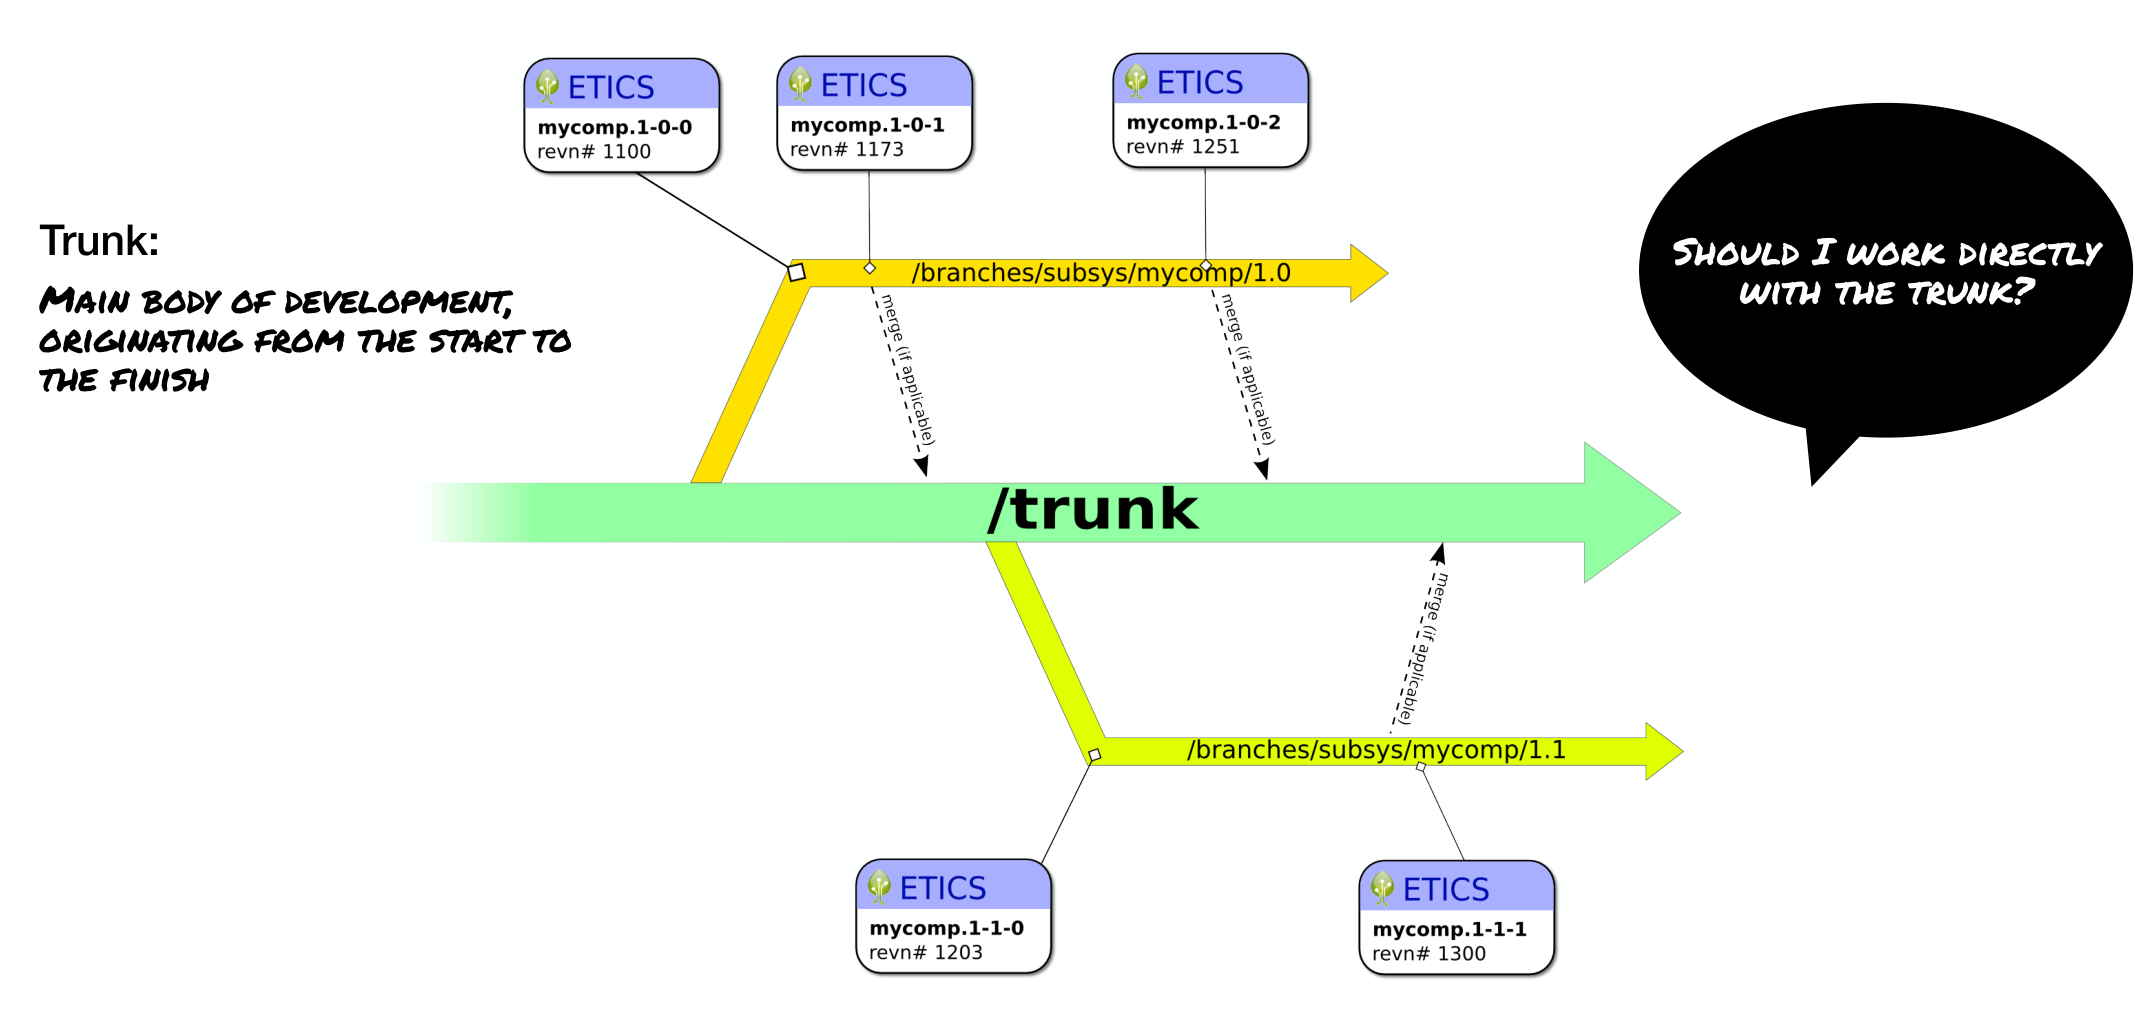
\includegraphics[width=\textwidth]{images/svn_trunk.png}
    \caption{Trunk in Subversion}
\end{figure}

\begin{figure}[H]
    \centering
    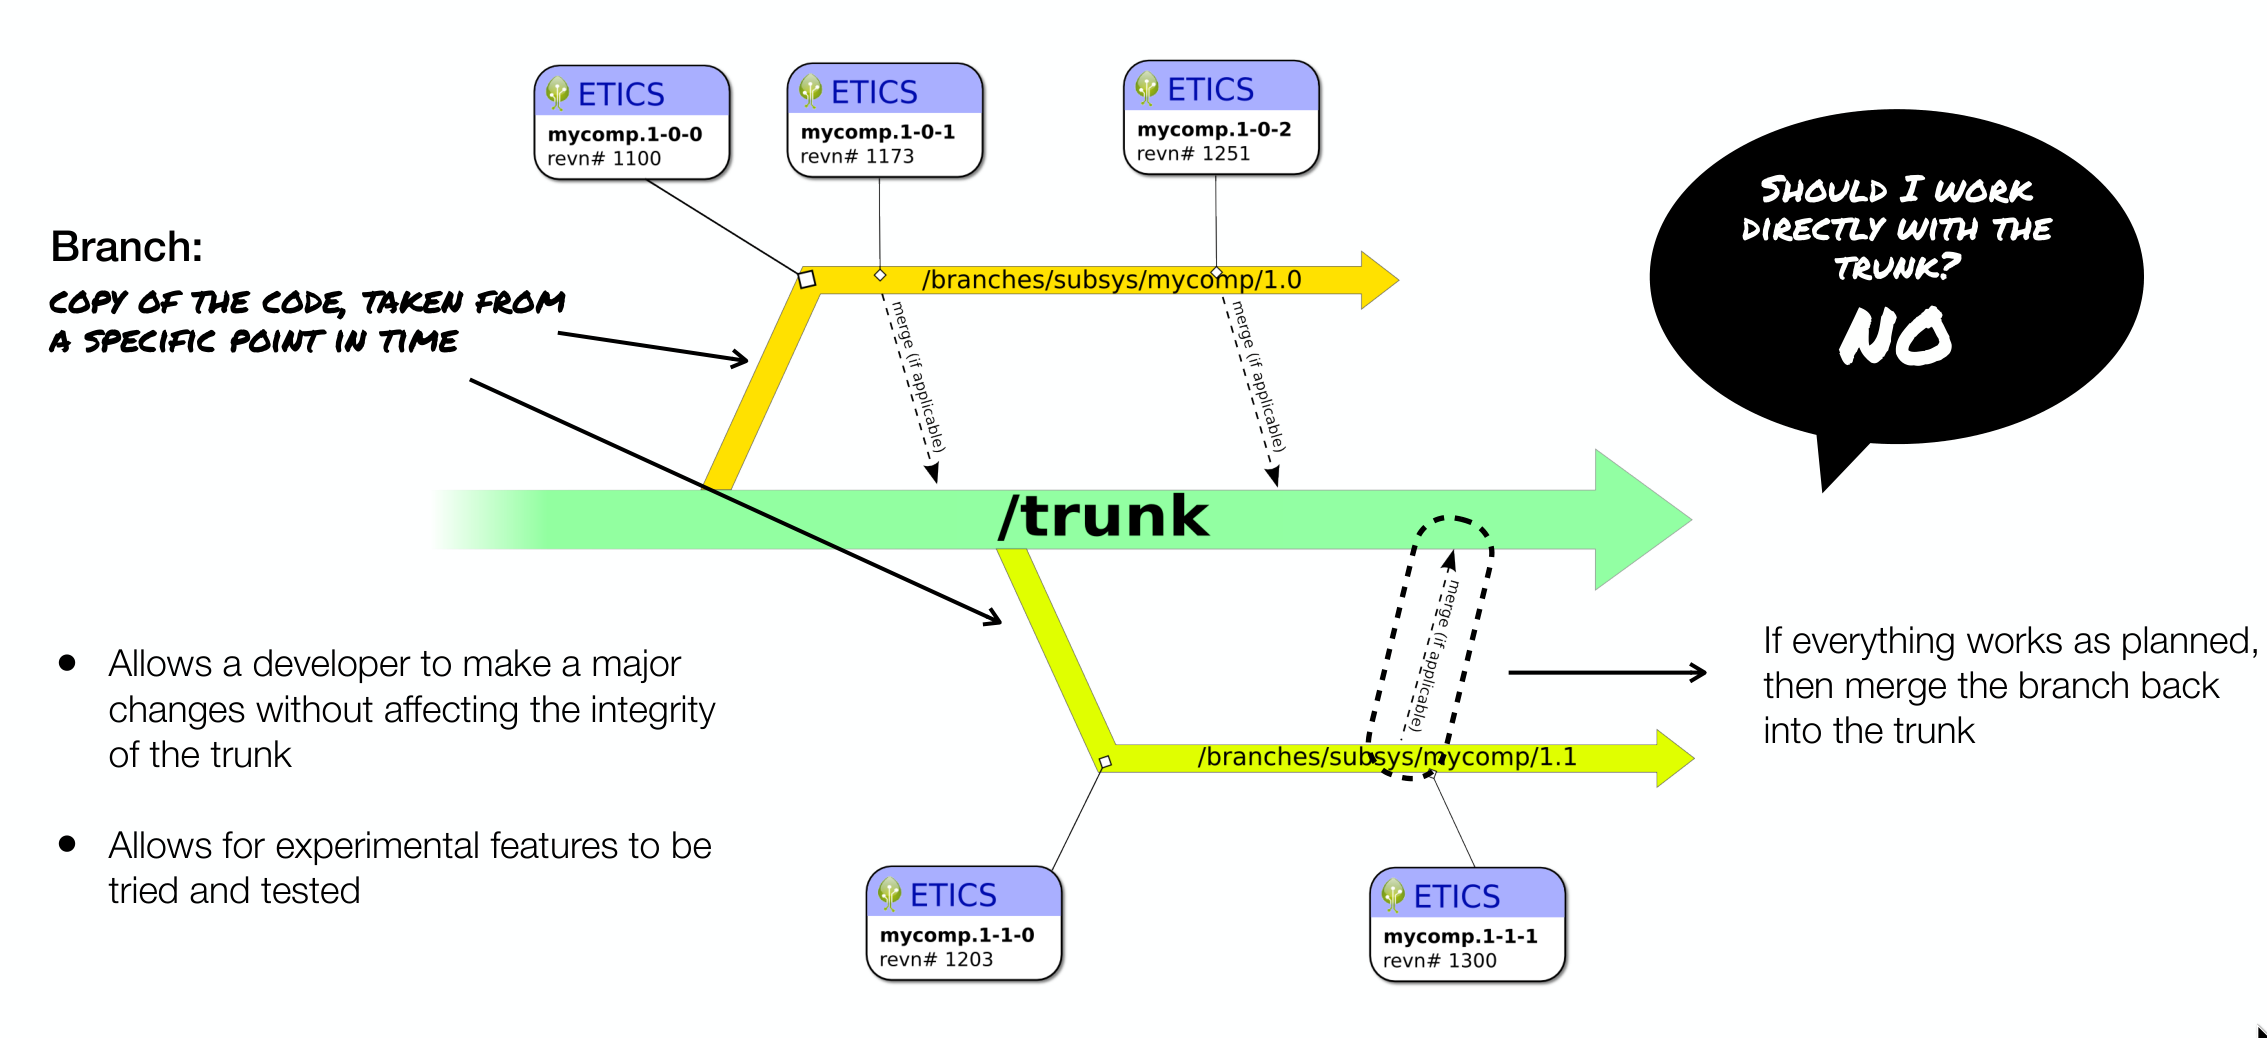
\includegraphics[width=\textwidth]{images/svn_branch.png}
    \caption{Branching in Subversion}
\end{figure}

When you check out the project in subversion, you will get the \verb|HEAD| revision.
When you invoke the command \mintinline{shell}{svn update}, you are updating your local copy to the \verb|HEAD| version
as well.
Branches should eventually be merged back into the trunk with \mintinline{shell}{svn commit}.
The trunk must build afterwards.
The commit is a process of storing changes from your private workplace to the central server.
After the commit, your changes are made available to the rest of the team;
other developers can retrieve these changes by updating their working copy.
Committing is an \textbf{atomic operation}: either the whole commit succeeds, or it is entirely rolled back -- users never
see a half-finished commit.

\begin{figure}[H]
    \centering
    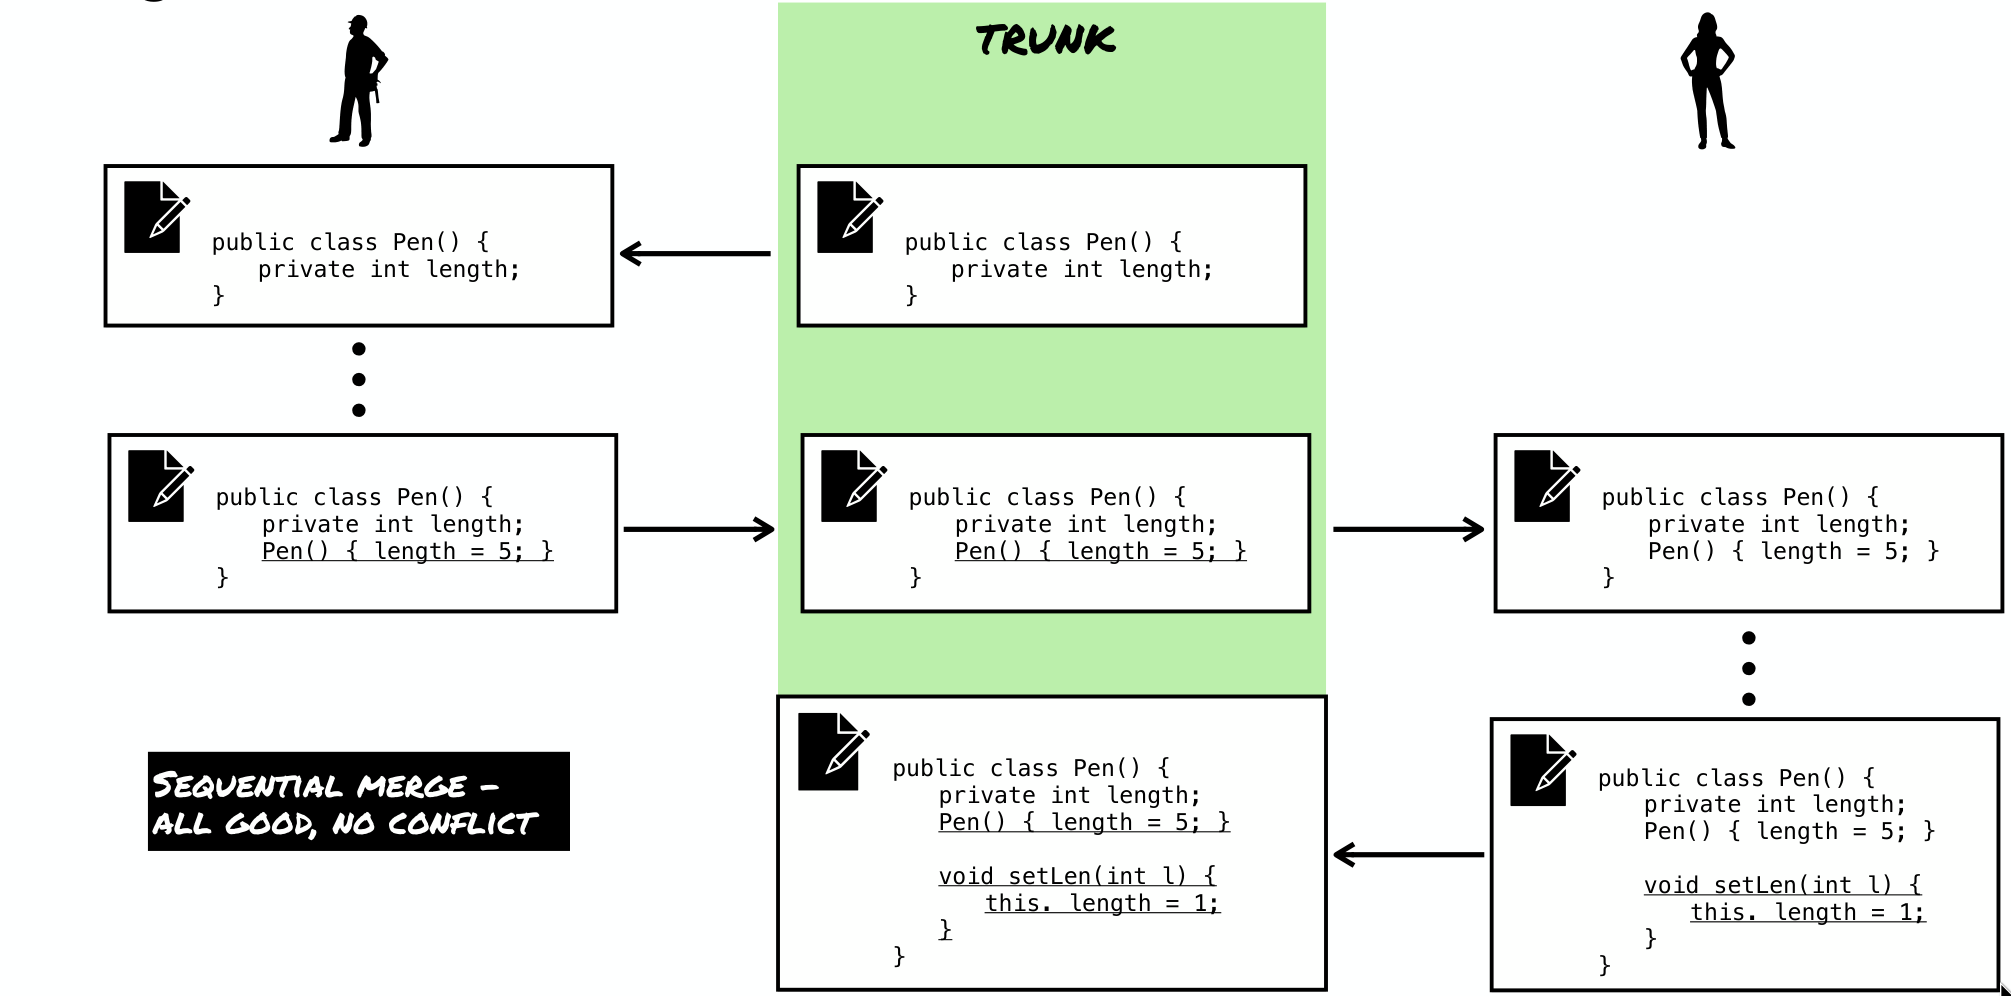
\includegraphics[width=0.8\textwidth]{images/svn_sequential_merge.png}
    \caption{Sequential Merge in Subversion}
\end{figure}

\begin{figure}[H]
    \centering
    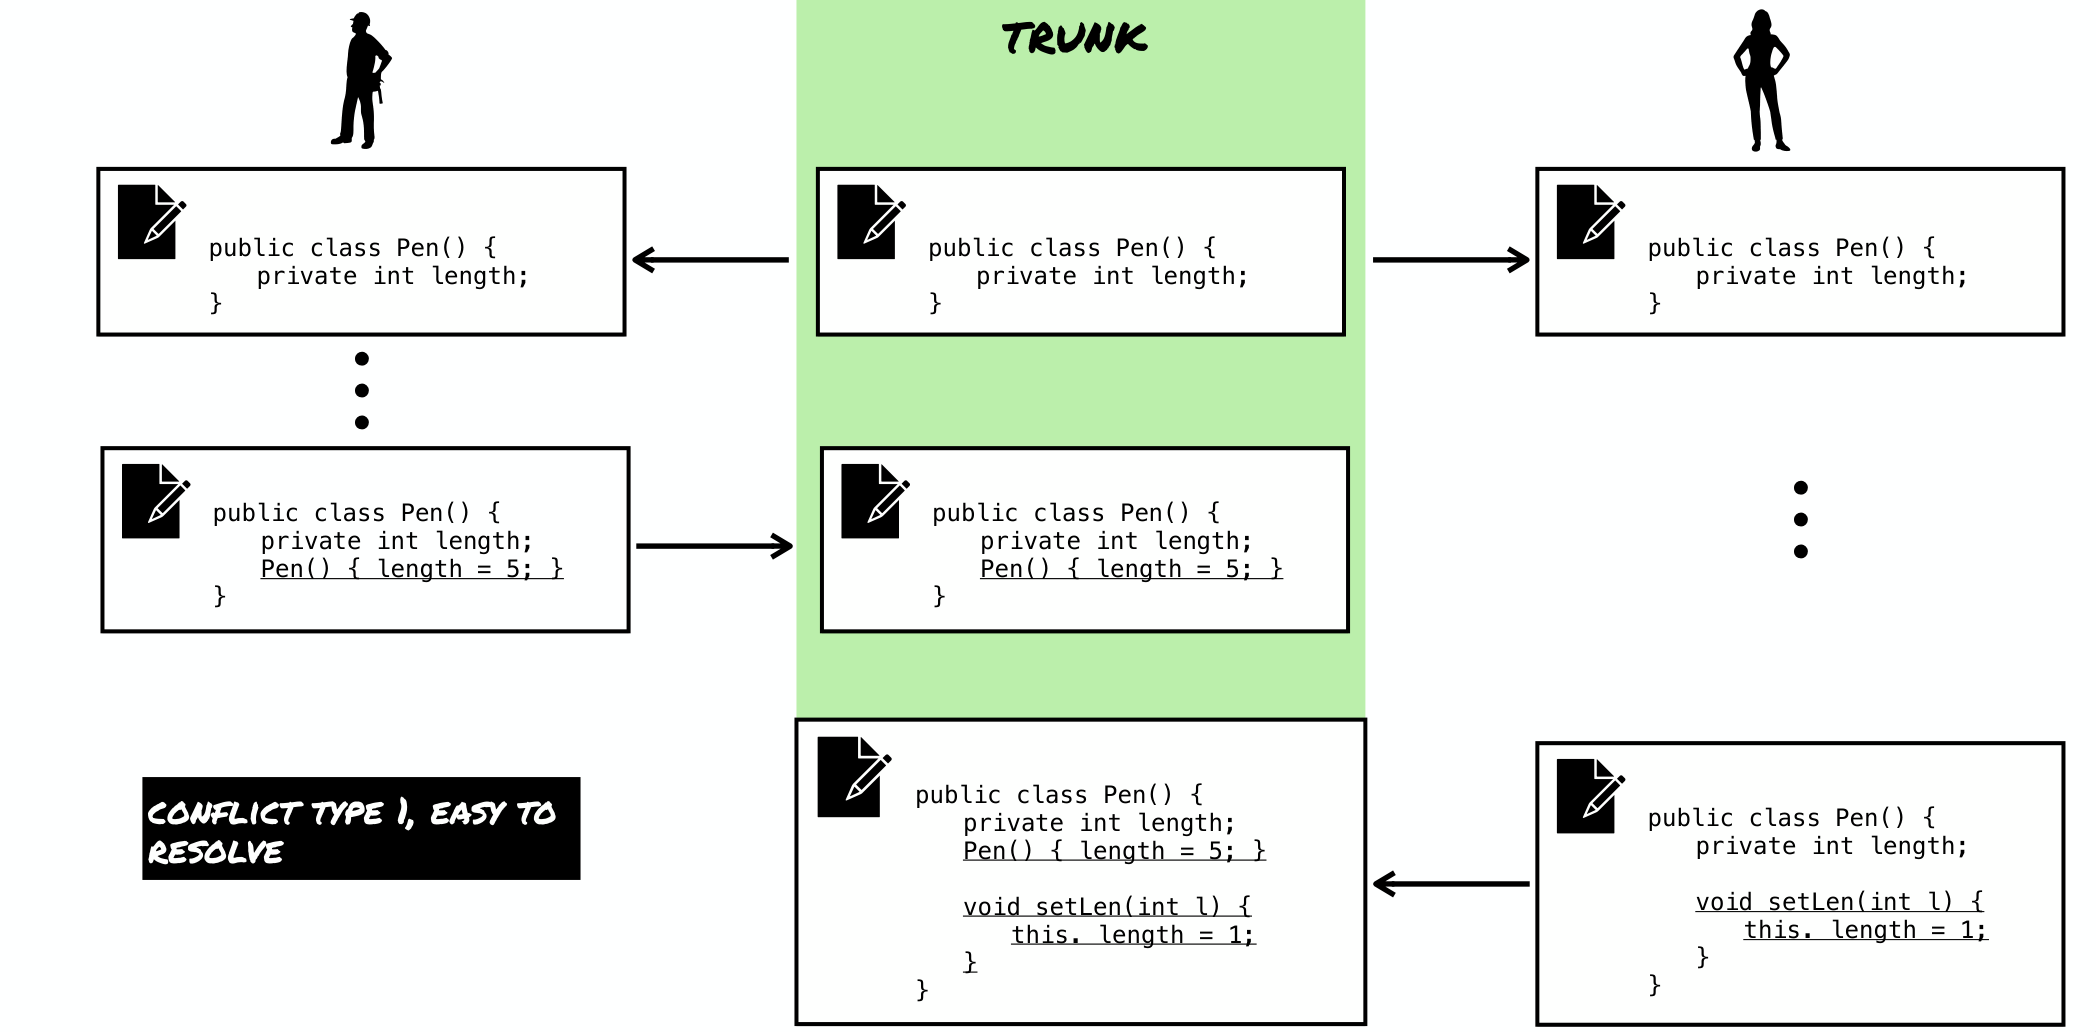
\includegraphics[width=0.8\textwidth]{images/svn_conflict1.png}
    \caption{Type 1 Merge Conflict in Subversion}
\end{figure}

\begin{figure}[H]
    \centering
    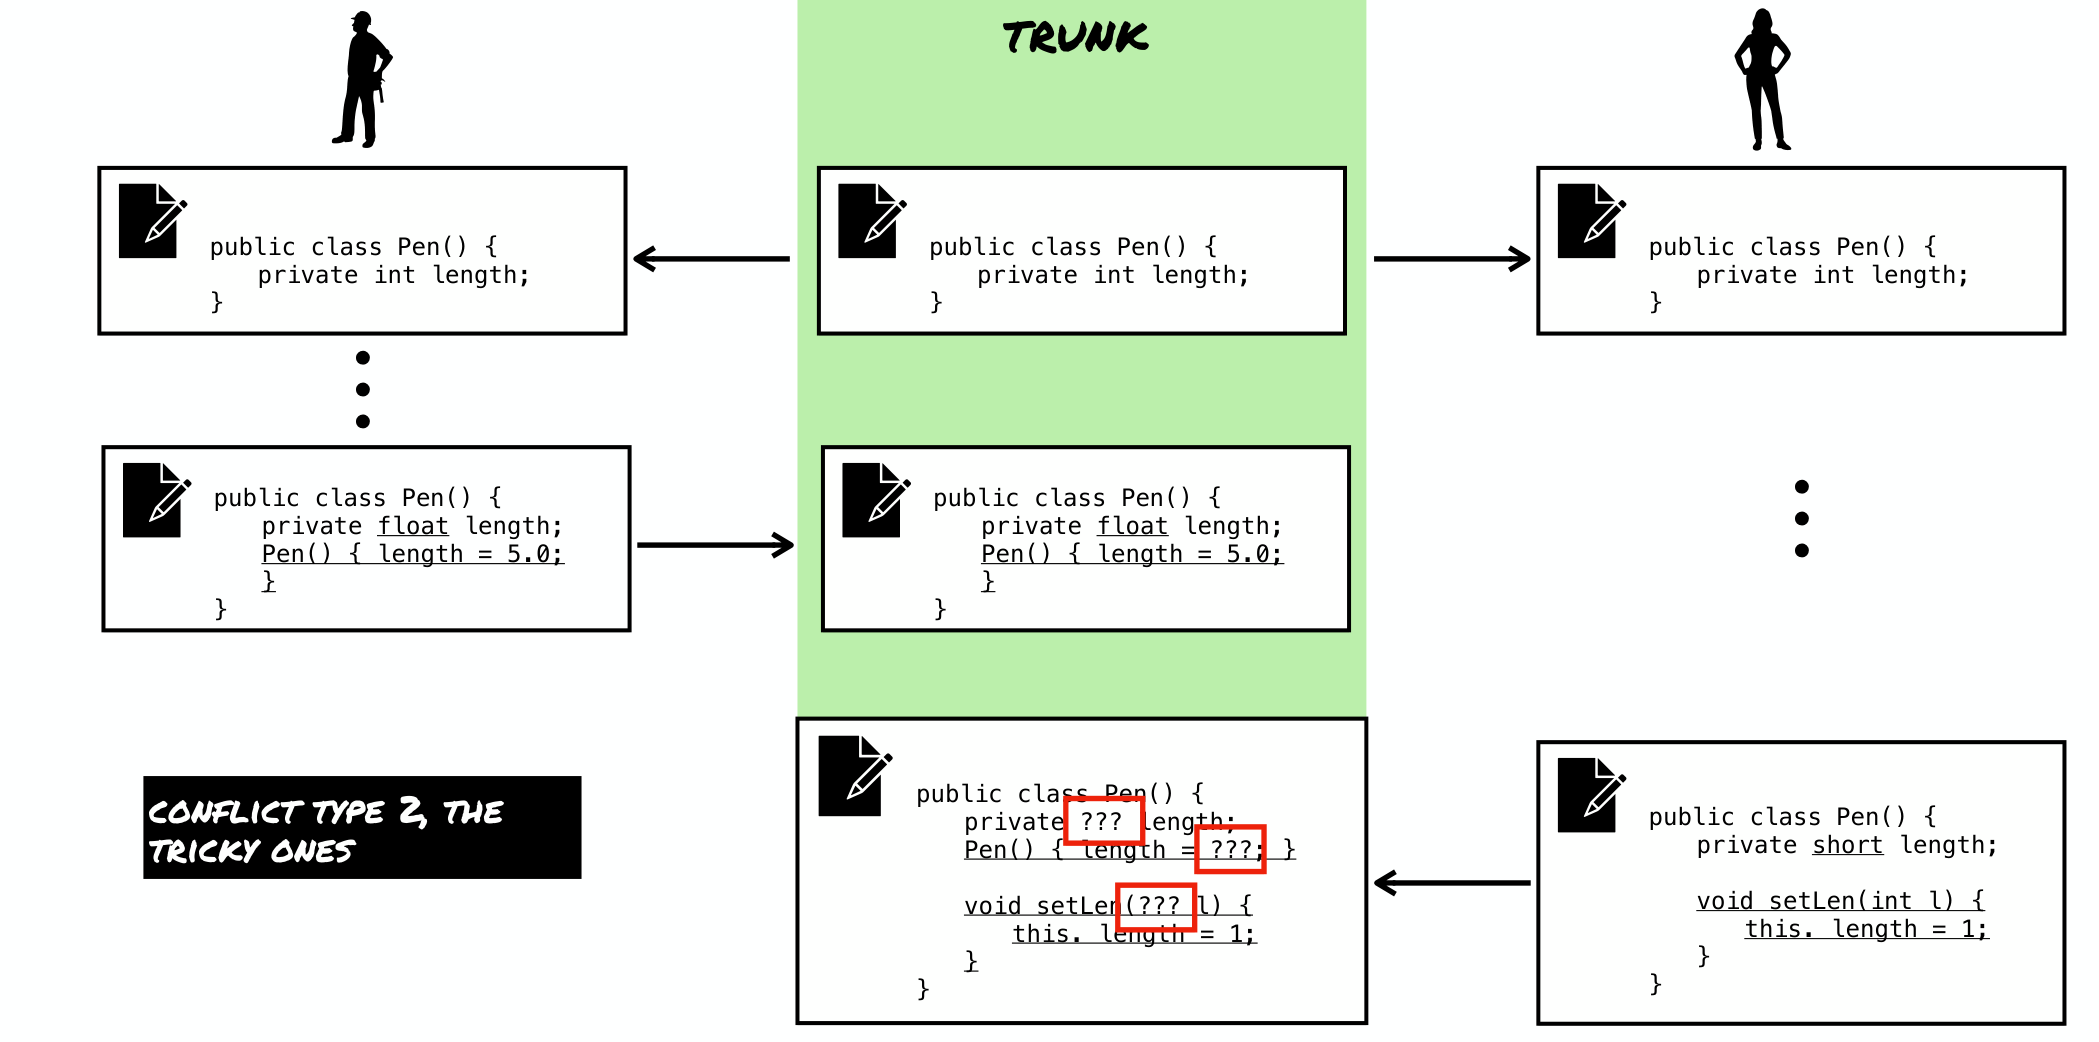
\includegraphics[width=0.8\textwidth]{images/svn_conflict2.png}
    \caption{Type 2 Merge Conflict in Subversion}
\end{figure}

\subsection{Distributed Version Control -- Git}
\begin{figure}[H]
    \centering
    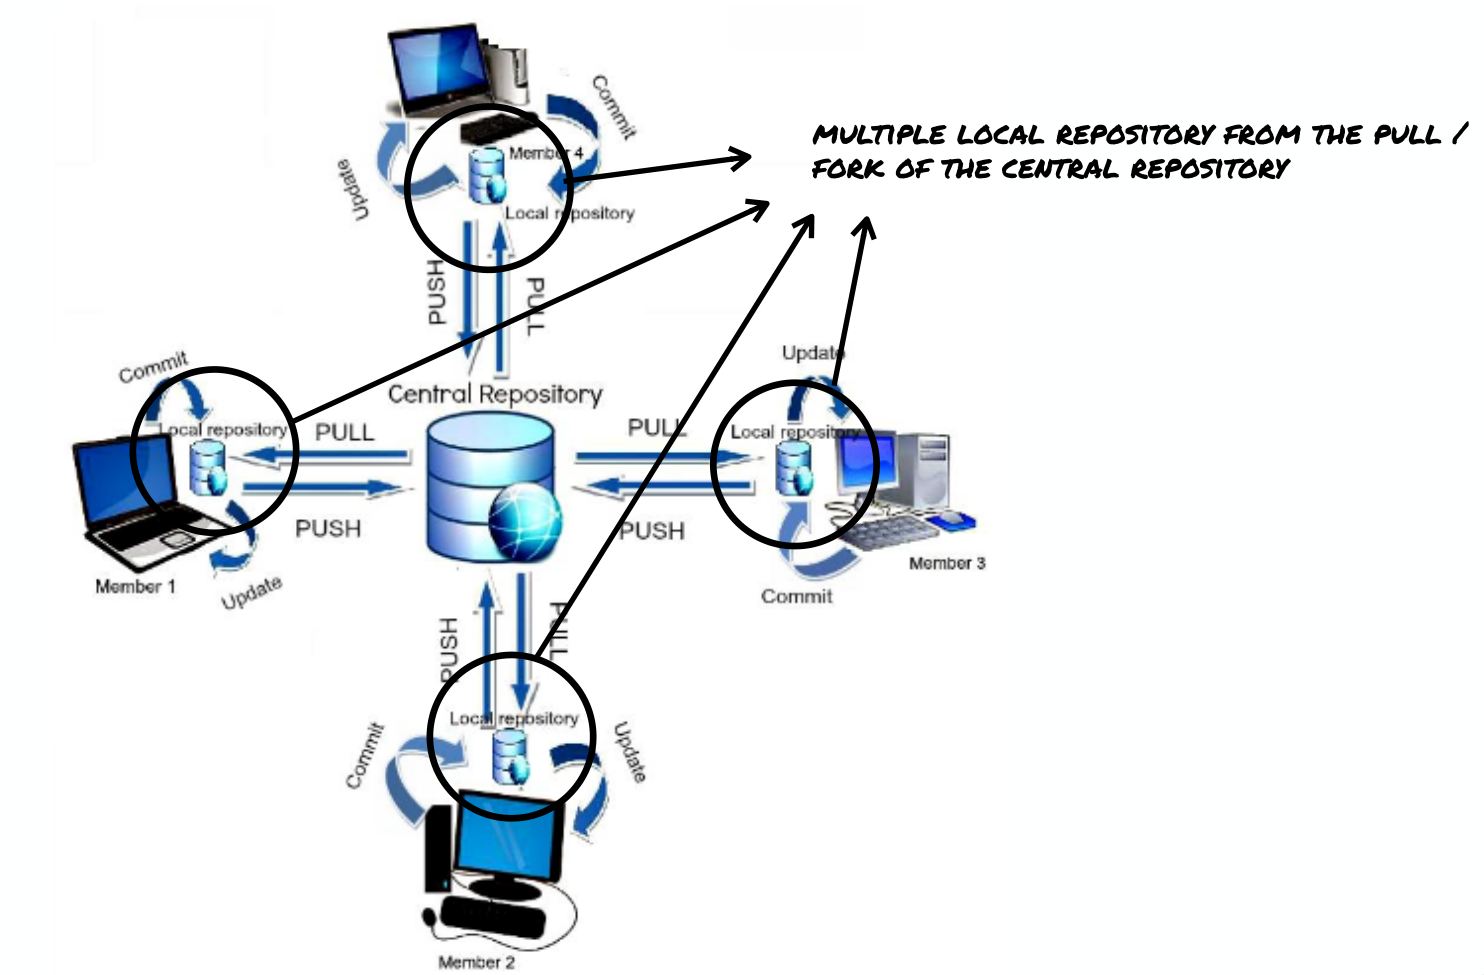
\includegraphics[width=\textwidth]{images/distributed_vcs.png}
    \caption{Distributed Version Control System Diagram}
\end{figure}

Git encourages branching for every feature, regardless of size.
After successful completion of the new feature, the branch is merged into the trunk.
Each developer gets their own local repository, meaning that developers don't need a network connection 
to commit changes, inspect previous version, or compare \verb|diff|s.
If the production trunk / branch is broken, developers can continue working uninhibited.

\subsubsection{GitHub}
\textbf{GitHub} is a web-based hosted service for Git repositories.
It allows you to host remote Git repositories and has a wealth of community-based services that makes it ideal for open-source projects.
It is a publishing tool, a version control system, \& a collaboration platform.

\subsubsection{Git Commands}
\begin{itemize}
    \item   \mintinline{shell}{git clone}: download (``clone'') the source code from the remote repository.
    \item   \mintinline{shell}{git fetch}: fetches the latest version from the repository that you've cloned but doesn't synchronise with all commits
            in the repository.
    \item   \mintinline{shell}{git pull}: pulls the latest version from the repository that you've cloned and synchronises with all commits
            in the repository. Equivalent to running \mintinline{shell}{git fetch} \& \mintinline{shell}{git merge}.
    \item   \mintinline{shell}{git push}: pushes the changes that you have committed to your local branch to the remote repository.
\end{itemize}

\subsubsection{Pull Requests}
A \textbf{pull request} is when you ask another developer to merge your feature branch into their repository.
Everyone can review the code \& decide whether or not it should be included in the master branch.
The pull request is an invitation to discuss pulling your code into the master branch, i.e. it is a forum for discussing changes.

\section{Build Tools}
\begin{figure}[H]
    \centering
    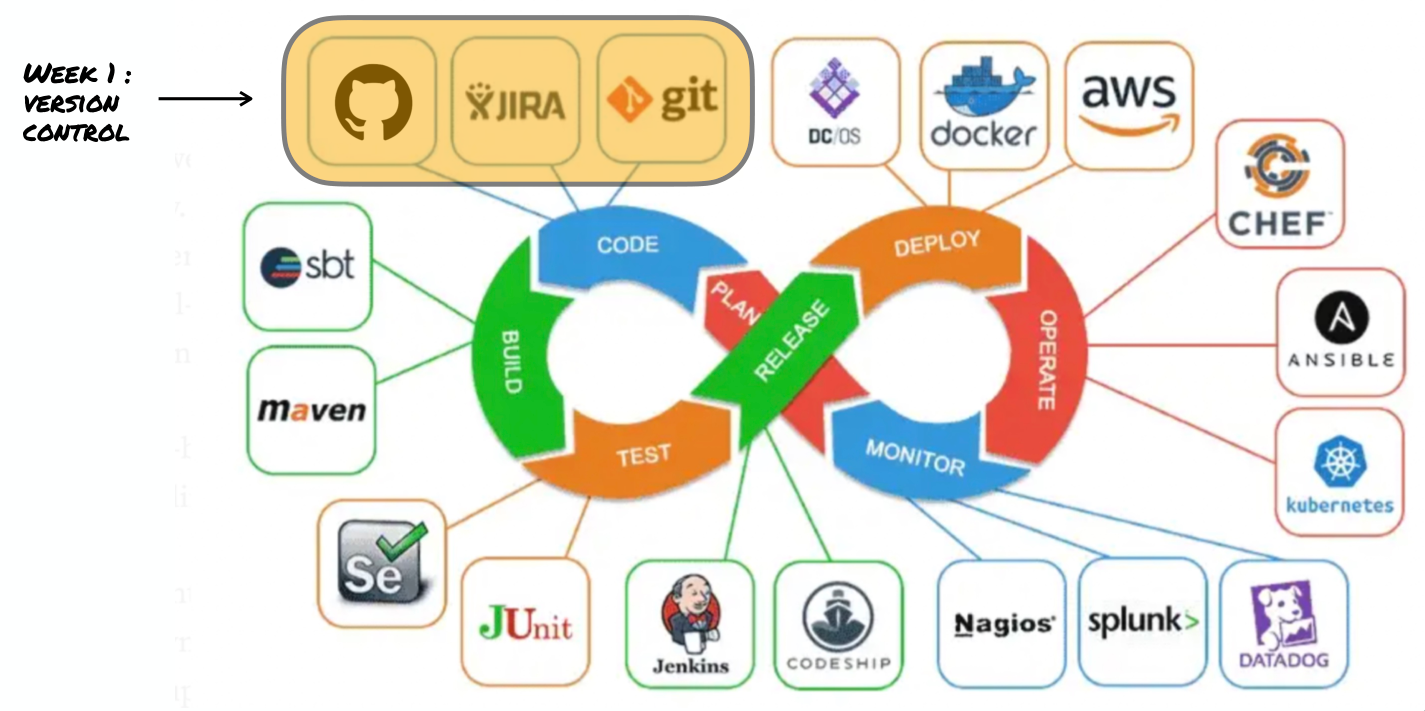
\includegraphics[width=\textwidth]{images/example_cd.png}
    \caption{Example of a Continuous Software Development System}
\end{figure}

The \textbf{build} is a process which covers all the steps required to create a deliverable of your software.
E.g., in Java:
\begin{enumerate}
    \item   Generating sources.
    \item   Compiling sources.
    \item   Compiling test sources.
    \item   Executing tests.
    \item   Packaging (\verb|.JAR|, \verb|.WAR|, \verb|EJB|).
    \item   Running health checks.
    \item   Generating reports.
\end{enumerate}

\textbf{Code Libraries} are convenient ways to package functionality \& reuse components.
E.g., \verb|JAR| files in Java or \verb|.DLL| files in Windows / \verb|.NET|.

\subsection{Maven}
\textbf{Maven} is a software build tool which can manage the project build, reporting, \& documentation.
All modern IDEs support Maven.
\begin{enumerate}
    \item   Compile source code.
    \item   Copy resources.
    \item   Compile \& run tests.
    \item   Package projects.
    \item   Deploy project.
    \item   Cleanup files.
\end{enumerate}

Developers wanted:
\begin{itemize}
    \item   to make the build process easy.
    \item   a standard way to build projects.
    \item   a clear definition of what the project consists of.
    \item   an easy way to publish project information and a way to share JARs across several projects.
\end{itemize}

The result is a tool that developers can use to build \& manage any Java-based project.
It embraces the idea of ``convention over configurations''.

\begin{figure}[H]
    \centering
    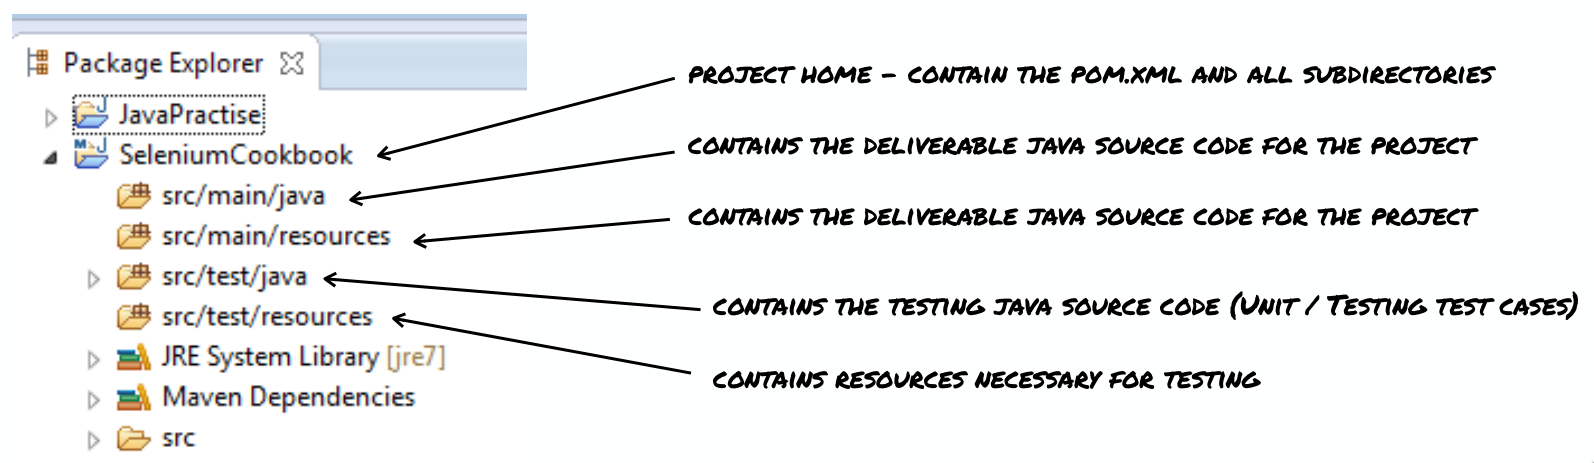
\includegraphics[width=\textwidth]{images/mvn_dir_structure.png}
    \caption{Maven Default Directory Structure}
\end{figure}

The command \mintinline{shell}{mvn package} compiles all the Java files, runs any tests, and packages the 
deliverable code \& resources into \verb|target/my-app-1.0.jar**|.
\\\\
The \verb|pom.xml| file is an XML document that contains all the information that Maven requires to automate 
a build of your software.
The \verb|pom.xml| is automatically updated on demand, but can be manually configured as well.
The POM provides all the configuration for a single project:
\begin{itemize}
    \item   General configuration covers the project's name, its owner, \& its dependencies to other projects.
    \item   One can also configure individual phases of the build process, which are implemented as plugins.
            E.g., one can configure the \verb|compiler-plugin| to use Java 1.5 for compilation, or specify
            packaging the project even if some unit tests fail.
\end{itemize}

Larger projects should be divided into several modules, or sub-projects each with its own POM.
All root POM can compile all the modules with a single command.
POMs can also inherit configuration from other POMs; all POMs inherit from the super-POM by default.
The super-POM provides default configuration, such as default source, default directories, default plugins,
etc.

\subsubsection{Plugins}
Maven build projects based on convention; it expects files to be in a certain place, which is very useful 
when developing in teams.

\begin{figure}[H]
    \centering
    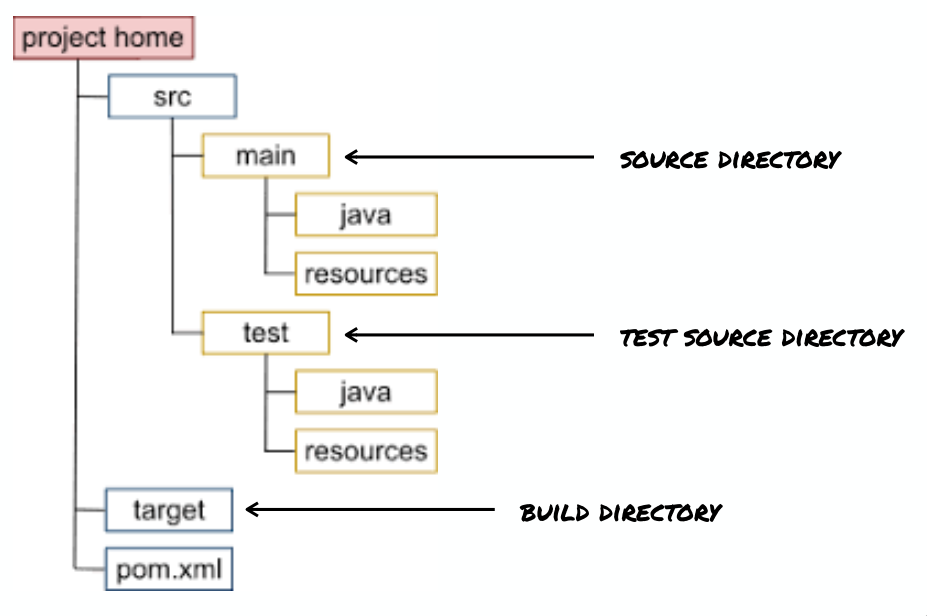
\includegraphics[width=0.7\textwidth]{images/mvn_conv_dir_structure.png}
    \caption{Maven Conventional Directory Structure}
\end{figure}

\begin{figure}[H]
    \centering
    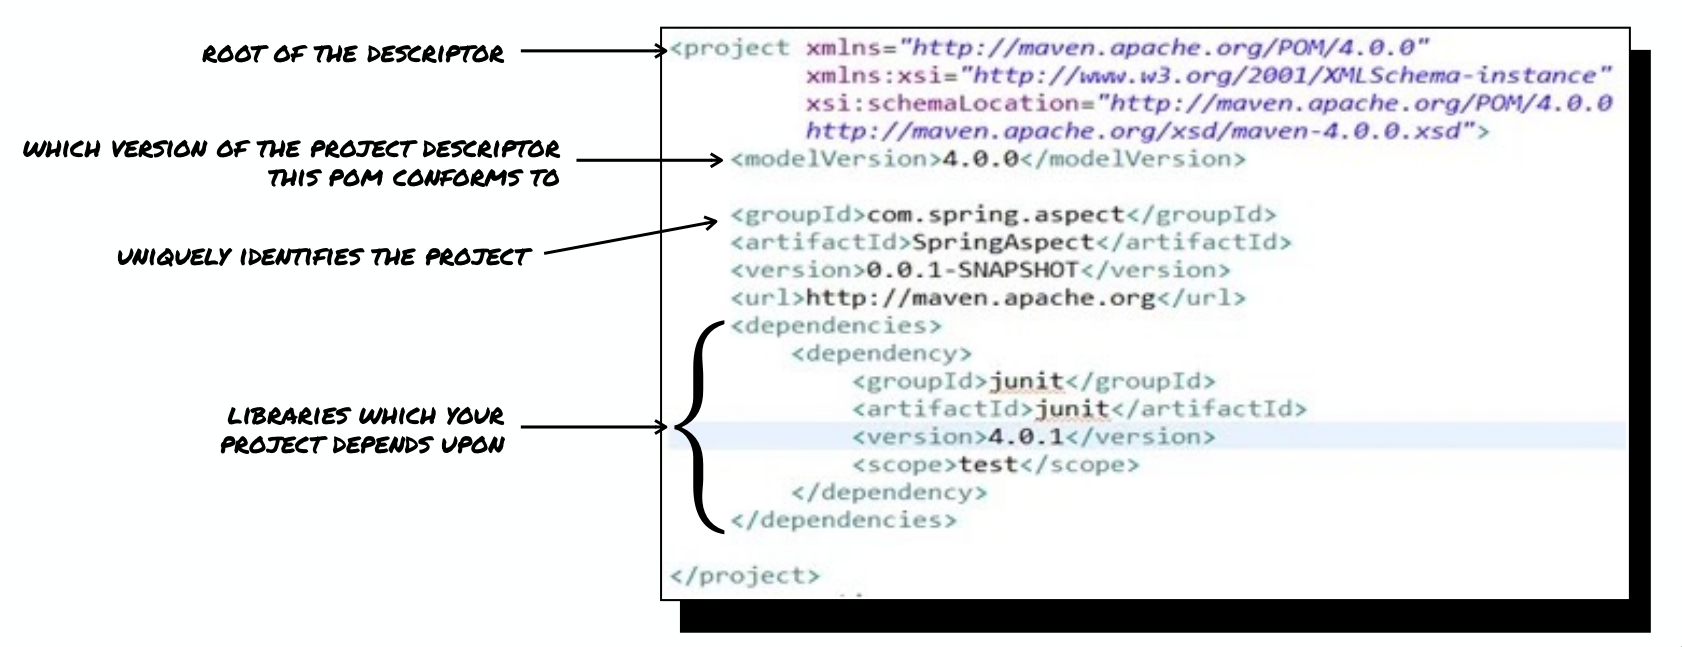
\includegraphics[width=\textwidth]{images/mvn_pom.png}
    \caption{Maven \texttt{pom.xml}}
\end{figure}

A Maven \textbf{plugin} is an extension or add-on module that enhances the functionality of Apache Maven.
Maven plugins provide additional capabilities \& tasks that can be executed during the build process or as part of 
project lifecycle management.
These plugins are typically packages as JAR (Java Archive) files and can be easily added to a Maven project's
configuration.
\\\\
The \textbf{core plugins} are plugins corresponding to default core phases (e.g., clean, compile).
They may also have multiple goals.

\subsubsection{Build Lifecycle}
The process for building \& distributing a particular project is clearly defined. 
It comprises a list of named phases that can be used to give order to goal execution.
Goals provided by plugins can be associated with different phases of the lifecycle.
e.g., by default, the goal \verb|compiler:compile| is associated with the compile phase, while the goal
\verb|surefire:test| is associated with the test phase.
\mintinline{shell}{mvn test} will cause Maven to run all goals associated with each of the phases up to \& including
the test phase.

\subsubsection{Dependency Management}
\textbf{Dependency management} is a central feature in Maven.
The dependency mechanism is organised around a co-ordinate system identifying individual artefacts such as software 
libraries or modules (e.g., JUnit).
If your project depends on a JAR file, Maven will automatically retrieve it for you, and store it in the user's local
repository.
If the JAR file depends on other libraries, Maven will ensure these are also included: these are known as 
\textbf{transitive dependencies}.
This wasn't always a part of Maven, so it's a huge benefit.
\\\\
Dependency management features supported include:
\begin{itemize}
    \item   Management: you can specify library version that transitive dependencies should use.
    \item   Scope: include dependencies appropriate for the current stage of the build, i.e., compile, test, run, etc.
    \item   Exclude dependencies: if project X depends on Project Y, and Project Y depends on Project Z, you can choose
            to exclude Project Z from your build.
\end{itemize}






\end{document}
